%step through each section of the atlas detector
%could spend more time on the muon spectrometer (like the new EE A-side detectors)
%and more time on the muon trigger
%Clare put in the minimal detail (no more than 20 pages) while Jeremy had 50 pages
%I could maybe fit somewhere in between

%need to define Muon Spectrometer (MS)
%need to define Inner Detector (ID)
%Assumptions:
%Will describe trigger


%I need to define things here like eta, pt, deltaR, etc 
%I may need to talk about isolation here
The ATLAS detector~\cite{ATLAS} is designed to measure
the products of the particle collisions produced by the LHC.
In particular, the detector seeks to measure those stable 
(or metastable) particles whose decay lifetime is sufficiently
long enough to interact with the detector.  This includes
a variety of fundamental particles (like muons) as well as 
composite particles (like neutrons). The wide variety of 
particles to be measured requires the implementation
of several sub-detector systems that work in tandem 
to identify and measure the properties of these particles.
The products of the LHC collisions travel in all directions, 
thus if there is any hope to measure all of the products of the collision
the detector must completely surround the collision point. 
The symmetry of the LHC dictates a cylindrically symmetric
shape for the ATLAS detector around this point.
There is another reason to build the detector to enclose
the collision point, since 
even with such a detector, the vanishingly small
cross-section of the neutrinos, which are also products
of the collision, means that these ghostly particles
will inevitably go undetected. But there is still hope!
If all other particles are measured, 
the presence of the neutrinos can be inferred 
using momentum constraints, as will be discussed later.  
In this way, the ATLAS detector is most generally suited
for measuring the wide variety of processes produced
by the LHC. 

\begin{figure}[ht!]
\centering
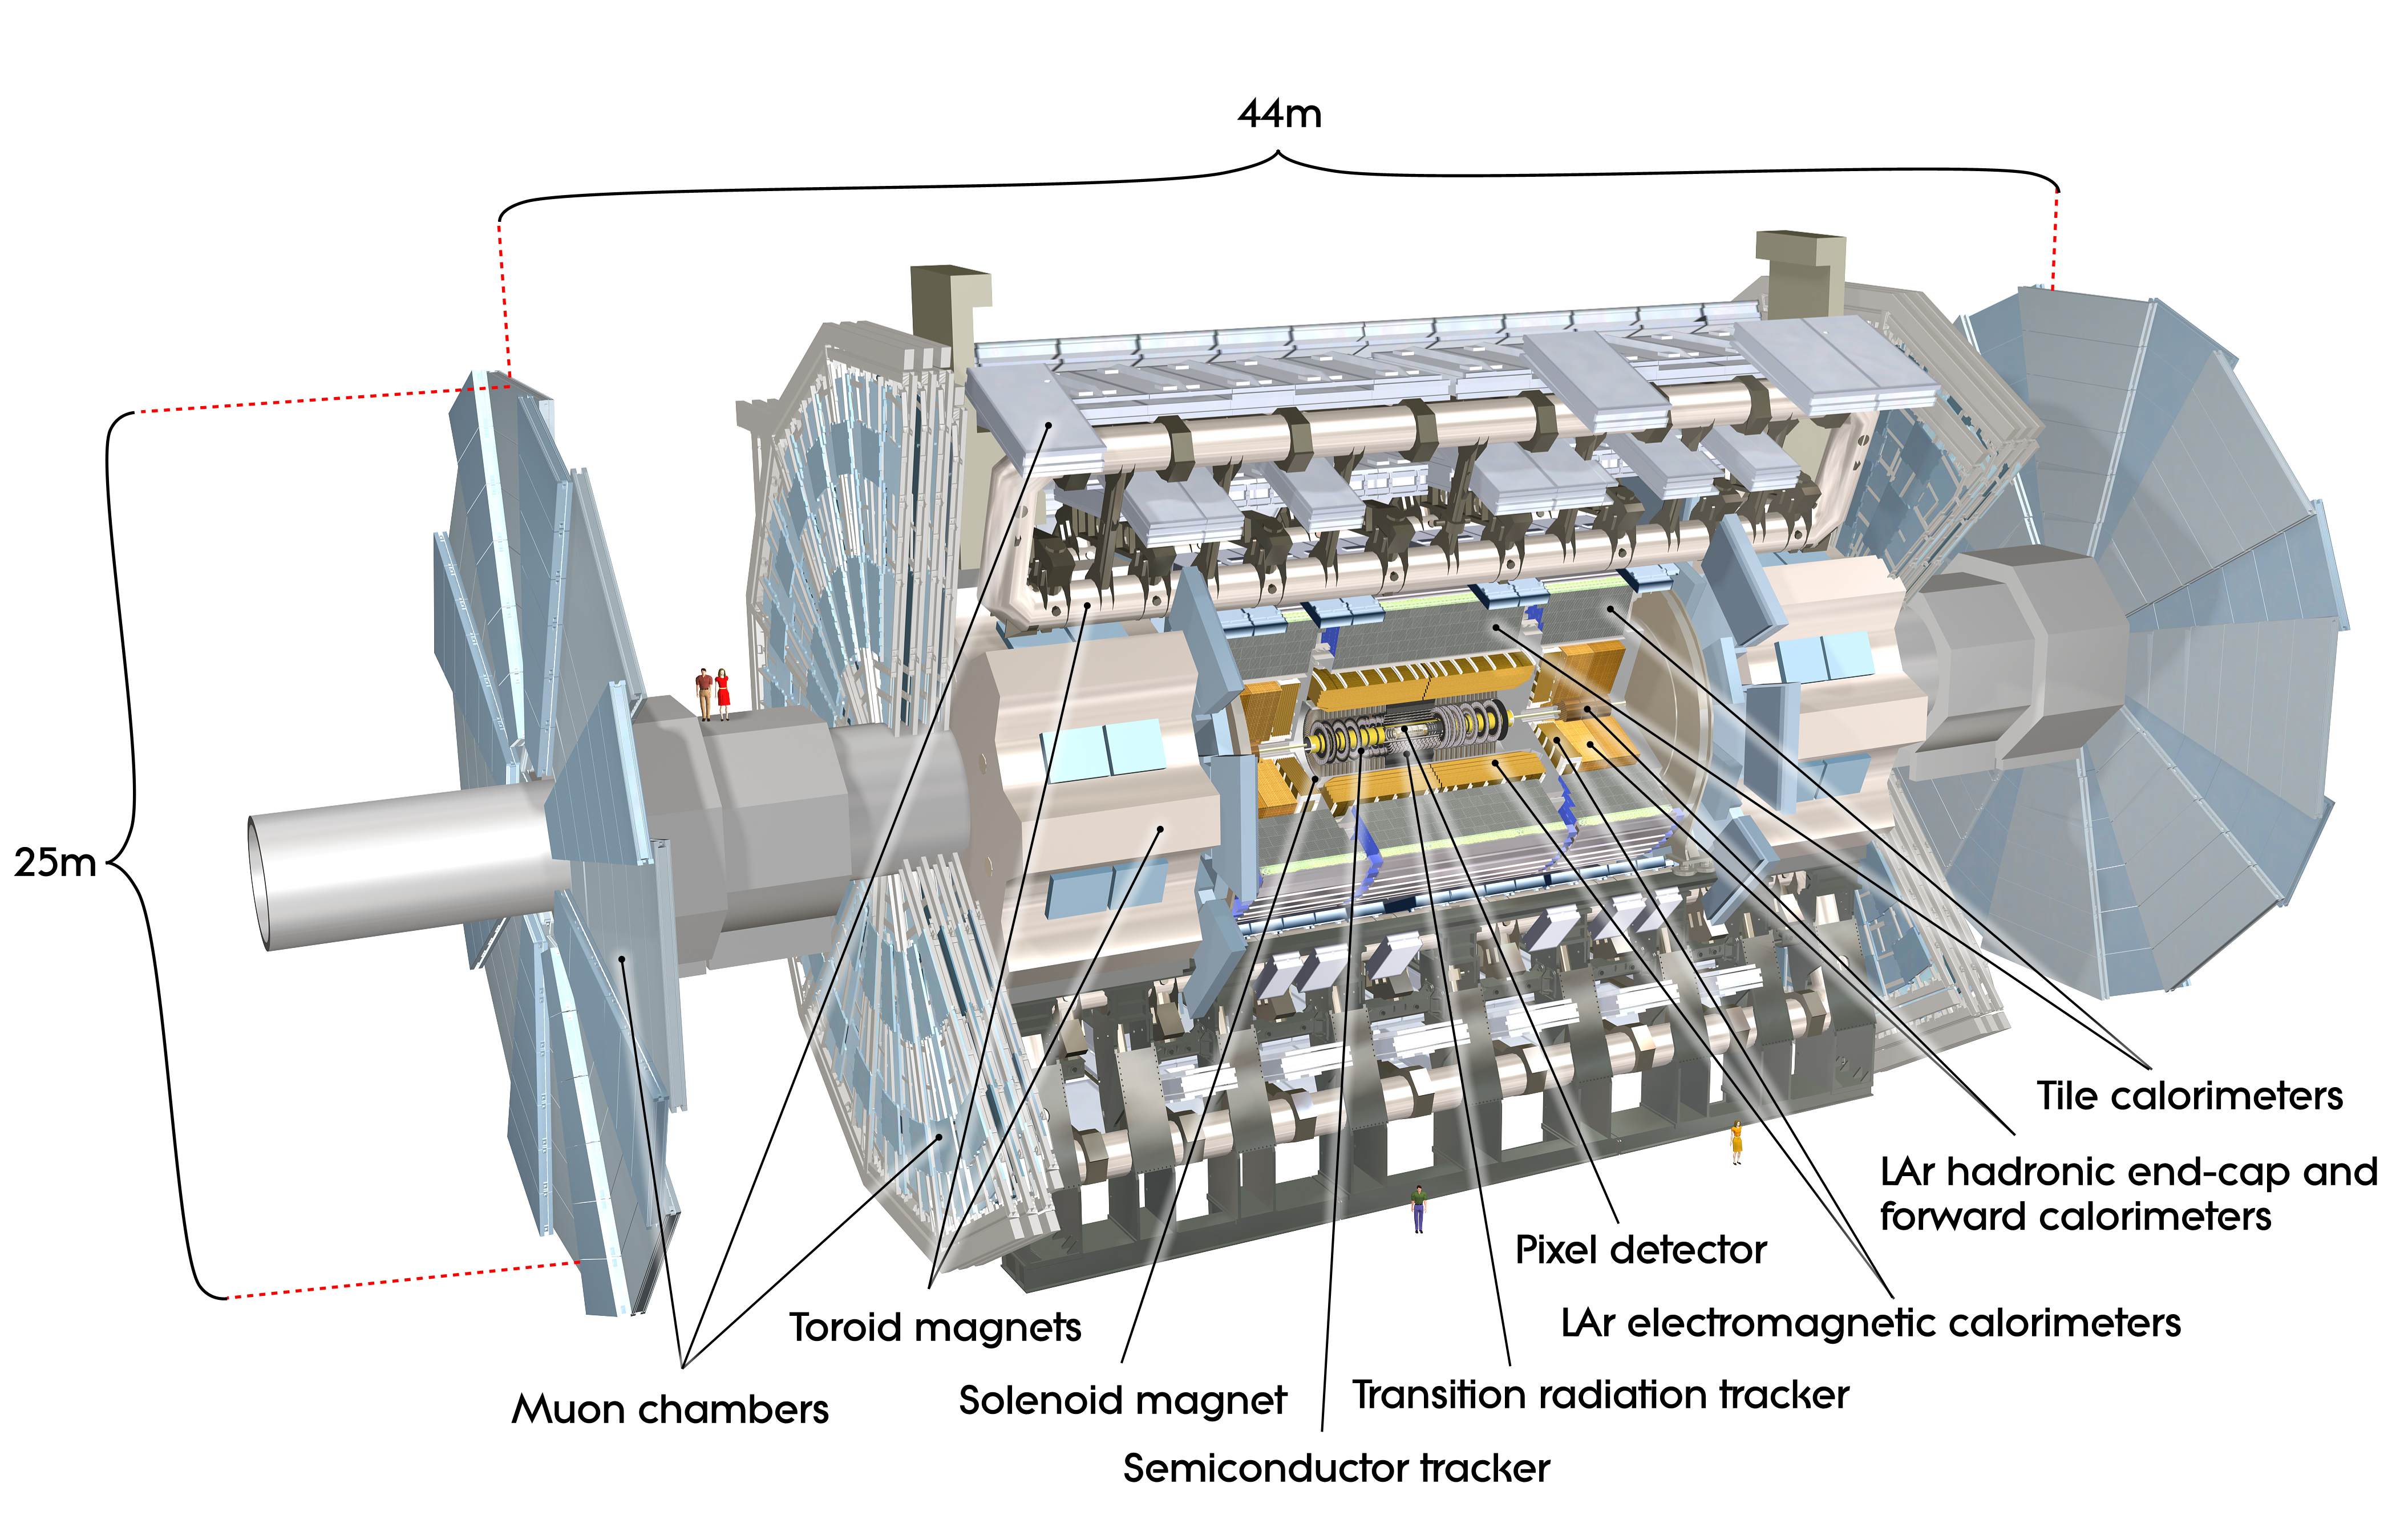
\includegraphics[width=.9\textwidth]{figures/atlas/detector.jpg}
\caption{A diagram of the ATLAS detector where the detector has
been artifically opened up to reveal the LHC beam line and the
various sub-detector components within. The sub-detector components
are labelled as such.}
\label{fig:atlas}
\end{figure}

A diagram of the ATLAS detector can be seen in \fig\ref{fig:atlas}.
It has a clearly cylindrical shape with a diameter of 25 meters
and length of 44 meters. The detector is massive, weighing
in at roughly 7000 tons; but it is also highly granular, with
over 100 million electronic channels that are arranged very precisely, 
in many cases on the order of tens of microns.
In the ``opened'' view of \fig\ref{fig:atlas}, the proton-proton
collisions from the LHC occur at the center core of the detector
and the sub-detector components build up around this point.
The detectable products of the collision pass outward from the collision
point through the different components where their energy and momentum
are measured. The way in which the particles interact with the various
sub-detector systems helps to identify the types of 
particles produced.
This can be more clearly seen in the diagram of 
\fig\ref{fig:atlas_wedge}, which shows how the most predominant
products of the LHC collisions interact with the different
components of the ATLAS detector.
Nearest the collision point is the inner detector (ID), designed to 
measure the paths of charged particles passing through using several
different subsystems. This 
is surrounded by a 2 Tesla solenoidal magnetic field which 
bends the trajectory of the charged particles by an amount
inversely proportional to the particle momentum, thereby allowing
for a momentum measurement.  Beyond that is the calorimeter system
which measures the energy deposits of all particles passing 
through (except for muons and neutrinos) by stopping them in their 
tracks. The calorimeter system 
itself is divided up into two components: the electromagnetic (EMCAL)
and hadronic calorimeter (HCAL) systems.
The EMCAL is situated in front of the HCAL and is designed
primarily to stop fundamental particles like electrons and photons
through ionization (?). The HCAL then is designed to stop
composite particles like protons and neutrons through (?).
Surrounding the carlorimeter system is the muon spectrometer (MS),
which is the largest component of the ATLAS detector and the one
that determines its size. It is designed to measure the 
trajectory of muons through ionization as they pass through
and ultimately leave the detector. The MS is also composed of 
three large superconducting air-core toroid magnets with an 
average magnetic field of roughly 0.5 Tesla which allows for
a measurement of the muon momentum. The neutrinos 
pass through undetected.

\begin{figure}[ht!]
\centering
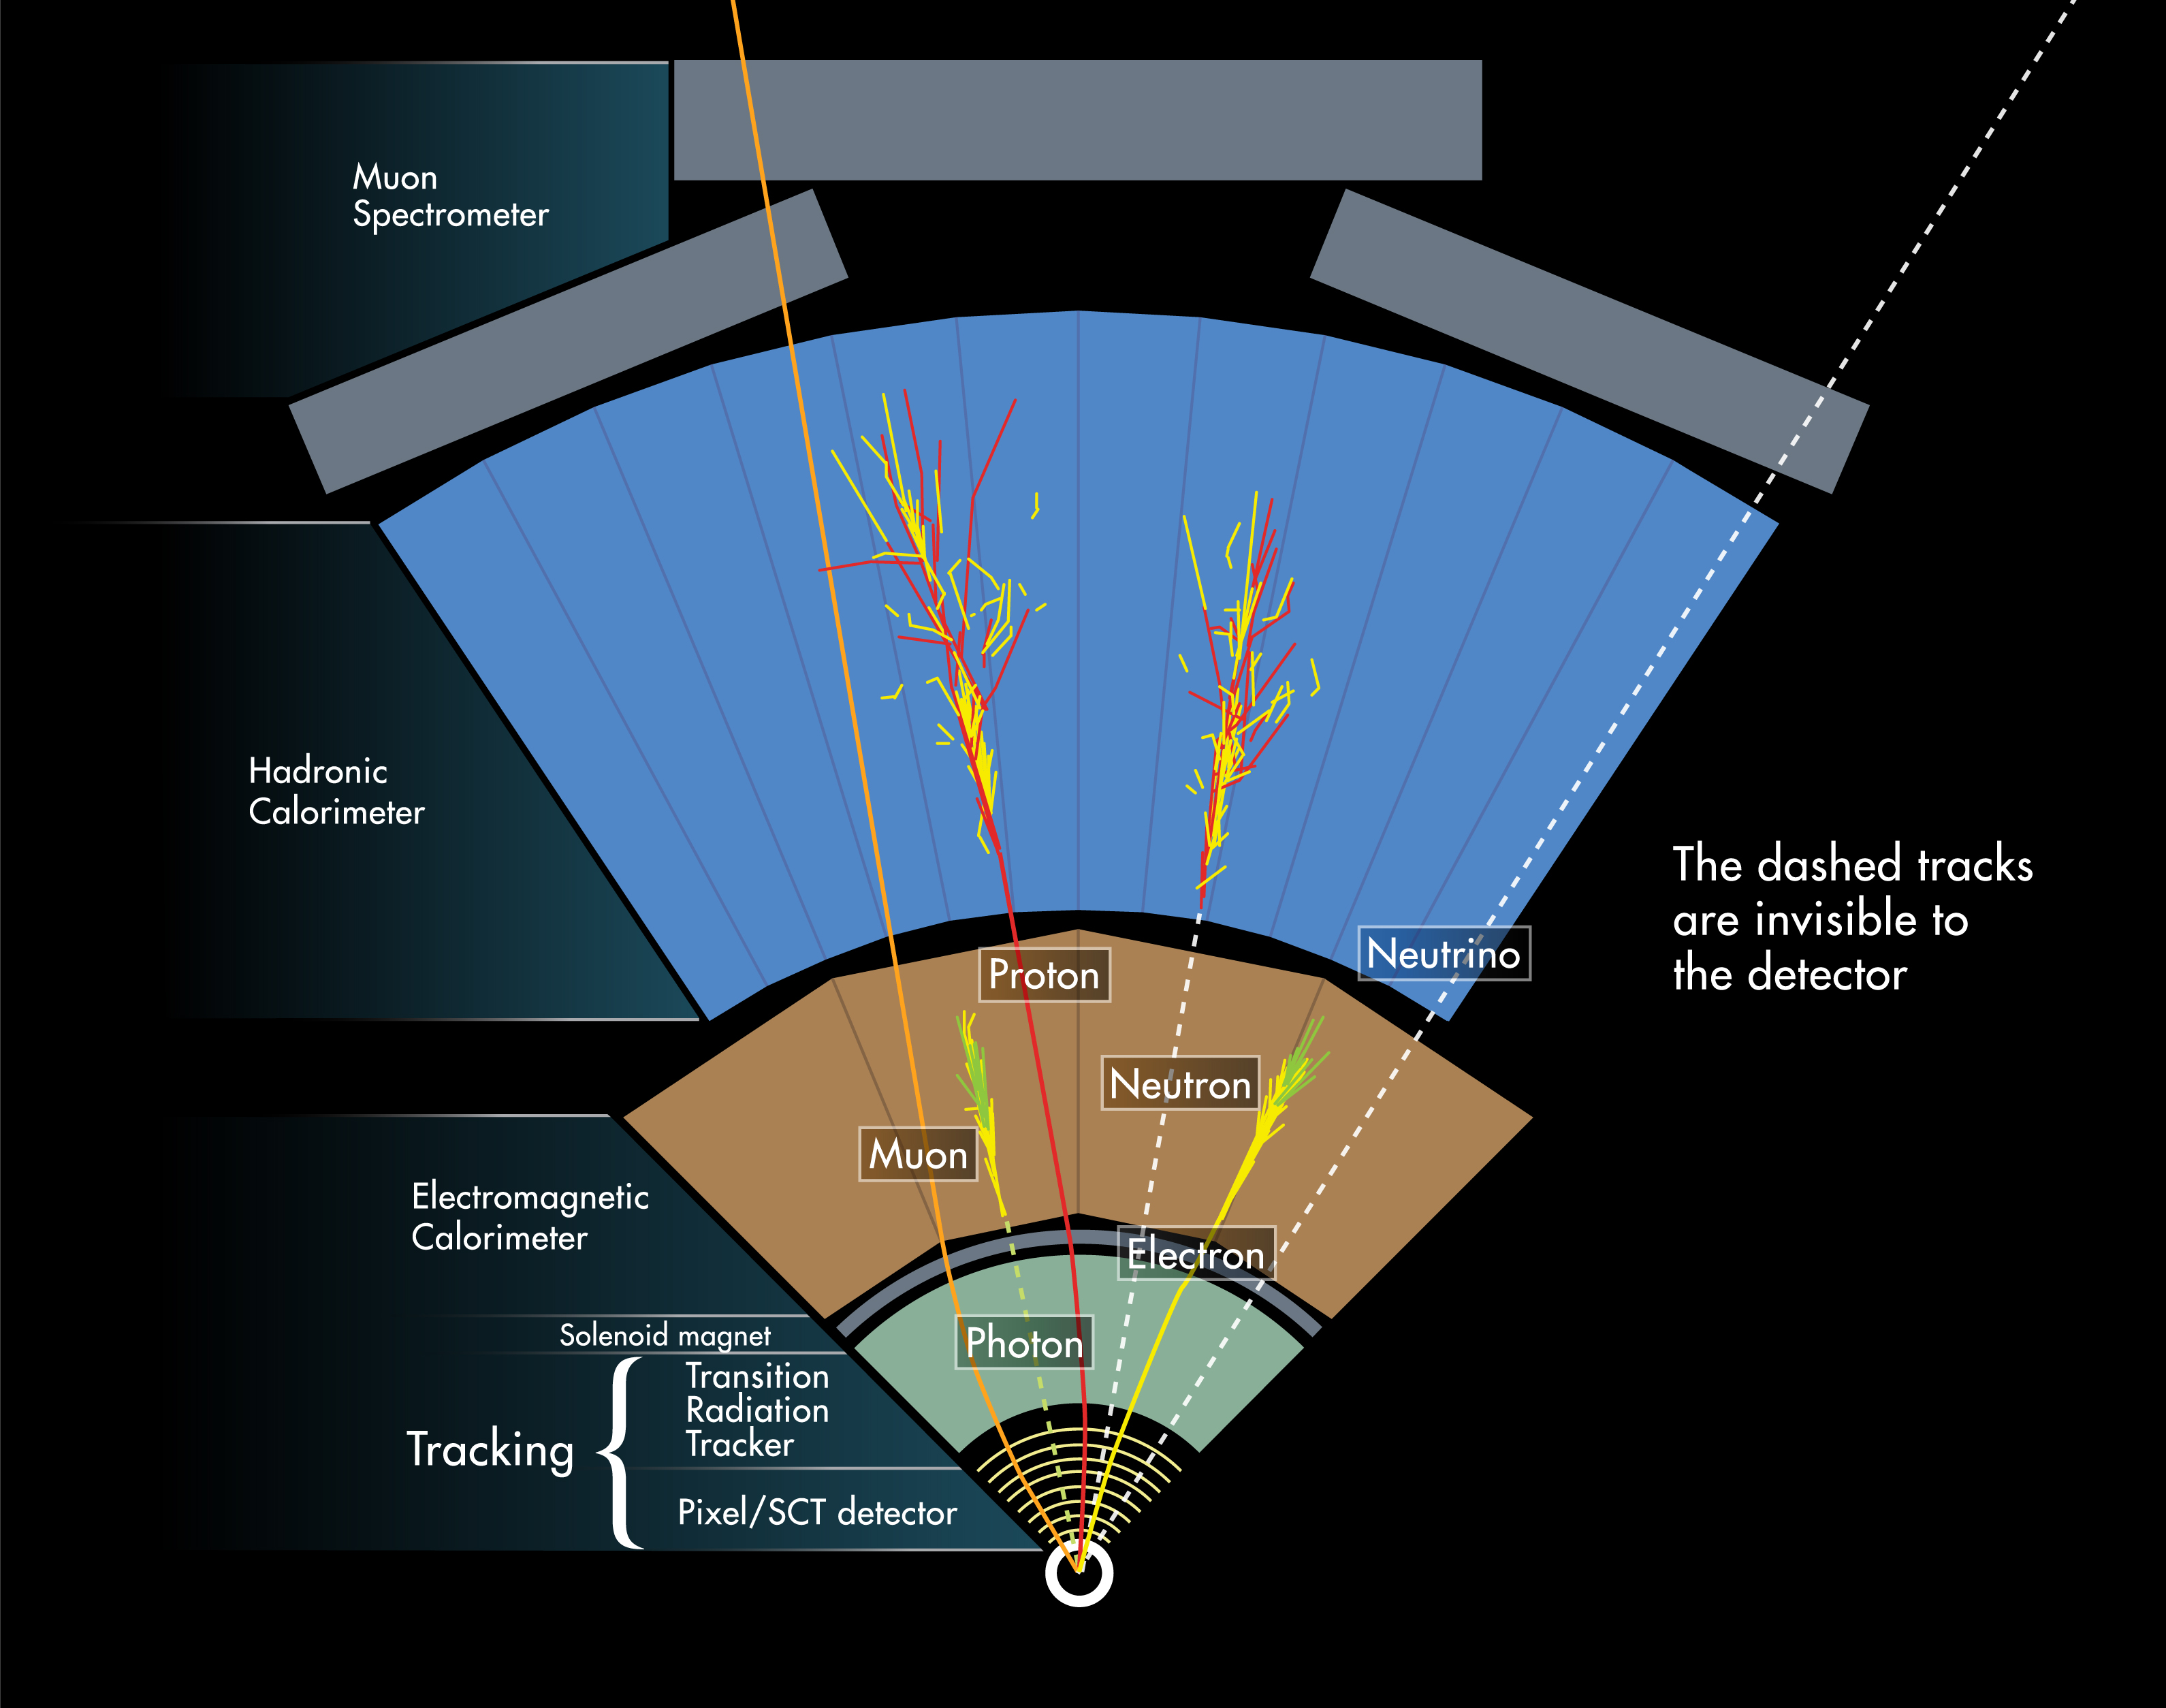
\includegraphics[width=.9\textwidth]{figures/atlas/wedge.jpg}
\caption{A diagram of one wedge of the ATLAS detector
as viewed from looking down the beam line. 
The sub-detector components are shown along with the 
particles that most predominately come from the collision.
The paths of the particles indicate how each particle typically 
interacts with the detector.}
\label{fig:atlas_wedge}
\end{figure}

The geometry of the ATLAS detector is defined using a 
right-handed cylindrical coordinate system with the $x$-axis
pointing inwards towards the center of the LHC ring, the $y$-axis point
up, and the $z$-axis pointing along the beamline.
The $x$ vs $y$ plane, which is perpendicular to the beamline,
is referred to as the transverse plane and typically 
defined using cylindrical coordinates with $r$ being the distance
from the center and $r$ being the azimuthal angle.
For describing the direction of the particle with respect 
to the beamline, a quantity called the pseudo-rapidity, $\eta$, is commonly
used
\begin{equation}
\eta = -\ln \tan (\theta/2) 
\label{eq:pseudorapidity}
\end{equation}
which is a function only of the polar angle, $\theta$, which 
itself is defined
as the direction of the particle with respect to the positive $z$-axis.
Changes in the pseudorapidity are 
invariant under Lorentz transformations along
the $z$-axis in the limit that the particle is approximately massless. 
As a result, its distribution is typically flat over
a wide range of pseudorapidity. At the LHC, most stable particles 
are produced with energies much larger than their mass, making the 
massless approximation valid.
The ATLAS detector has nearly uniform $2\pi$ coverage in $\phi$,
while in $\eta$ the ID is restricted to $|\eta| < 2.5$,
the MS to $|\eta| < 2.7$, and the calorimeter systems all the way
to $|\eta| < 4.9$.

The total momentum of the proton-proton collision in the transverse
plane is zero. Since the detector has full azimuthal coverage 
in the transverse plane, we can test this constraint by measuring
the total momentum from the particles measured in the detector.
The magnitude of a particle's momentum 
in the transverse plane is referred to as the 
transverse momentum, $\pt$.
Thus, we may refer to this constraint as
\begin{equation}
\Bigg| \sum_{i\in\textrm{All Particles}} \vec{p}_{\textrm{T},i} \Bigg| = 0
\end{equation}
where the transverse momentum is added vectorially and then
the magnitude is taken.
After adding up the $\pt$ of all of the particles to obtain
the total transverse momentum, 
any imbalance with respect to this constraint
is referred to as the
missing transverse energy, $\met$, and is attributed to the 
neutrinos produced in the collision. 
There is no such constraint on the momentum along the $z$-direction
because the momentum fraction of the partons as taken
from the PDFs are not known with certainty. This is the case
even though the momentum along the $z$-direction of the 
protons from which the partons are taken is, in fact, known.
Thus there is no way of determining with certainty the 
momentum of the neutrinos in the $z$-direction.



\section{Inner Detector}
\label{sec:atlas_id}
%be sure to include material description of inner detector
%from ATLAS JINST paper: figures/atlas/DetectorPaper1.pdf 
%so that can refer to when discussing charge mis-id
\section{Calorimeters }
\section{Muon Spectrometer}
%do i want to talk about muon reconstruction?
%definitely mention muon resolution
\section{Trigger}

